\subsection{Контекстно-свободные грамматики}

Английское название этого термина -- ``context-free grammars''. Более правильно было бы перевести как "бесконтекстные грамматики" или "контекстно-независимые грамматики". Но так уж сложилось.

Мотивация введения КС-грамматик такая. У нас есть регулярные языки, которые очень просто распознавать: просто моделируем конечный автомат, но к сожалению, многие интересные языки автоматами не распознаются.

\begin{conj}
    Четверка $(\Sigma, N, R, S \in N)$, где $\Sigma$ --- алфавит (мн-во \textbf{терминалов}), $N$ --- конечное множество \textbf{нетерминалов}, $R$ --- конечное множество правил, $S$ --- стартовый нетерминал; называется \textbf{КС-грамматикой}, если:
    \begin{itemize}
        \item $\Sigma \cap N = \varnothing$
        \item Каждое правило имеет вид: $A \to r$, 
        где $A \in N$, $r \in (\Sigma \cup N)^*$ ($r$ может быть пустой).
    \end{itemize}
\end{conj}  

\textbf{Замечание.} Ещё правила иногда записывают в таком виде:
    $$ A \to u_0 B_1 u_1 B_2 u_2 \dots B_l u_l $$
где $A \in N$, $l \geqslant 0$; $u_0, \dots, u_l \in \Sigma^*$; $B_1, \dots, B_l \in N$.

\begin{conj}
    \textbf{Отношение выводимости за один шаг}. \\ 
    Пусть $\alpha, \beta \in (\Sigma \sqcup N)^*$. Тогда $\beta$ выводится из $\alpha$ за один шаг (обозначаем $\alpha \to \beta$), если:
    \begin{itemize}
        \item $\alpha = u A v$, где $u, v \in (\Sigma \sqcup N)^*$, $A \in N$
        \item Есть правило $A \to \gamma$ в $R$
        \item $\beta = u \gamma v$
    \end{itemize}
\end{conj}

\begin{conj}
    \textbf{Отношение выводимости за несколько шагов}.
    $$ \alpha \to_n \beta \text{ если } \exists \gamma : \alpha \to_{n-1} \gamma, \; \gamma \to \beta $$
\end{conj}

\begin{conj}
    \textbf{Отношение выводимости} вообще.
    $$ \alpha \to_* \beta \text{ если } \exists n : \alpha \to_n \beta $$
\end{conj}

\begin{conj}
    \textbf{Язык, задаваемый КС-грамматикой} $(\Sigma, N, R, S)$ --- это множество строк $\beta \in \Sigma^*$, т.ч. $S \to_* \beta$.
\end{conj}

Более неформально: строка распознаётся КС-грамматикой, если её можно вывести из начального нетерминала, причём сама строка нетерминалов не содержит. 

А отношение выводимости здесь определяется совершенно естественно и очень похоже на то, что у нас было в ассоциативном исчислении: просто применяем правила и получаем новые строки. 

А применить правило значит просто взять и заменить соотв. нетерминальный символ на строку.

Возникает вопрос. Мы же доказали, что выводимость как в одностороннем, так и в двустороннем ассоциативном исчислении алгоритмически неразрешима. А что в данном случае? На самом деле, правила КС-грамматик гораздо более ограничены, чем правила ассоц. исчисления. Позже мы поймём, что таких ограничений достаточно для алгоритмической разрешимости. 

\textbf{Пример.} Язык Дика --- правильные скобочные последовательности:
\begin{gather*}
    \bigg(\Sigma = \{ (, ) \}, \quad N = \{ S \}, \quad R = \{ S \to (S), \; S \to S S, \; S \to \varepsilon \}, \quad S \bigg)
\end{gather*} 
Правильные скобочные последовательности (ПСП) можно определить по индукции:
\begin{itemize}
    \item пустая строка является ПСП;
    \item конкатенация двух ПСП --- ПСП, т.е. строка вида $ut$, где $u,t$ --- ПСП;
    \item ПСП, завёрнутая в скобки --- ПСП, т.е. строка вида $(u)$, где $u$ --- ПСП.
\end{itemize}
Теперь нетрудно понять по этому определению, что все ПСП распознаются:
\begin{itemize}
    \item $\varepsilon$ выводится по третьему правилу
    \item $ut$ можно получить так: по второму правилу за один шаг получаем $S S$, а потом из первого символа выводим $u$, а из второго выводим $t$
    \item $(u)$ можно получить похожим способом: сначала за один шаг по первому правилу получаем $(S)$, а потом из $S$ выводим $u$.
\end{itemize}
Причём любая выводимая из $S$ строка, не содержащая нетерминалов, является ПСП. Это можно доказать индукцией по длине строки.

Из всех этих определений становится понятно, почему символы из алфавита называются терминалами, а символы из $N$ нетерминалами: по правилам заменять можно только нетерминалы; с другой стороны, как только у нас в строке появился терминал, он оттуда никуда не денется; и вывод строки из языка нельзя считать завершённым, пока в строке есть хоть один нетерминал.

\begin{conj}
    \textbf{Дерево вывода} (дерево разбора) --- подвешенное дерево, т.ч. все дети упорядочены, в каждом узле записан какой-то символ $c_v$ или пустая строка $\varepsilon$, при этом в корне записан начальный нетерминальный символ $s$, и для любой вершины $v$ верно одно из двух:
    \begin{itemize}
      \item $c_v$ --- терминальный или в $v$ записана пустая строка. Тогда $v$ --- лист.
      \item $c_v$ --- нетерминальный. Тогда есть какое-то правило для текущего $c_v \rightarrow \alpha$, т.ч. если $\abs{\alpha} \geqslant 1$, то у вершины $v$ $\abs{\alpha}$ сыновей, в каждом из которых записан соответствующий ему символ из $\alpha$, иначе у $v$ один ребёнок, в котором записана пустая строка.
    \end{itemize}

    Мы говорим, что некоторое дерево вывода $T$ --- \textbf{дерево вывода для строки $\alpha$}, если $\alpha$ получается конкатенацией слева направо всех символов и пустых строк в листьях $T$.
\end{conj}

\textbf{Пример.} Дерево вывода для строки $()()()$: \\
\begin{center}
    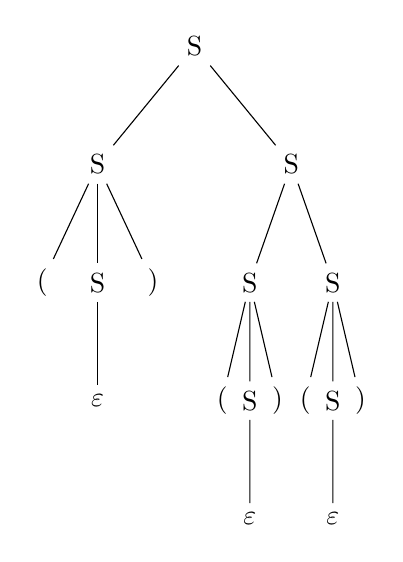
\begin{tikzpicture}[sibling distance=7em,
        every node/.style = {align=center}]]
        \node {S}
            child { node {S} 
                child [sibling distance=2em] { node {(} }
                child [sibling distance=2em] { node {S}
                    child { node {$\varepsilon$} }
                }
                child [sibling distance=2em] { node {)} }
            }
            child{ node {S}
                child [sibling distance=3em]  { node {S} 
                    child [sibling distance=1em] { node {(} }
                    child [sibling distance=1em] { node {S}
                        child { node {$\varepsilon$} }
                    }
                    child [sibling distance=1em] { node {)} }
                }
                child [sibling distance=3em]  { node {S} 
                    child [sibling distance=1em]{ node {(} }
                    child [sibling distance=1em]{ node {S}
                        child { node {$\varepsilon$} }
                    }
                    child [sibling distance=1em]{ node {)} }
                }
            }
            ;
    \end{tikzpicture}
\end{center}

\begin{conj}
    \textbf{Альтернативное определение языка, задаваемого КС-грамматикой.} Язык, задаваемый КС-грамматикой --- множество строк, для которых существует дерево вывода. 
\end{conj}

Нетрудно понять, что это определение тождественно старому.

\begin{conj}
    \textbf{КС-язык} --- язык, задаваемый некоторой КС-грамматикой.
\end{conj}

\begin{theorem}
    Пусть $L$ --- регулярный язык. Тогда $L$ --- КС-язык.
\end{theorem}
\begin{proof}
    Раз $L$ --- регулярный язык, то существует ДКА $(\Sigma, Q, q_0, \delta, F)$, его распознающий:
    \begin{itemize}
        \item $\Sigma$ --- алфавит;
        \item $Q$ --- множество состояний;
        \item $q_0 \in Q$ --- начальное состояние;
        \item $F \subset Q$ --- терминальные состояния;
        \item $\delta : Q \times \Sigma \to Q$ --- функция переходов. 
    \end{itemize}

    Построим по нему КС-грамматику $(\Sigma, N, S, R)$. Возьмём $N := Q$, $S := q_0$. Если в $\delta$ был переход $(q, a) \mapsto q'$, то добавим в $R$ правило $q \to a q'$. Если $q_f \in F$, то добавим правило $q_f \to \varepsilon$. 

    Нетрудно понять, что такая КС-грамматика задаёт тот же язык. По сути, она просто моделирует работу ДКА.
\end{proof}
\begin{conj}
    Правила такого вида:
    \begin{align*}
        q \to a q' && q_f \to \varepsilon
    \end{align*}
    называют \textbf{автоматными}. 
\end{conj}

Таким образом мы поняли, что класс КС-языков содержит класс регулярных языков. Следующий пример показывает, что КС-грамматики на самом деле расширяют класс регулярных языков.

\textbf{Пример.} $L = \{ a^n b^n \mid n \geqslant 0 \}$. Мы доказывали, что он не является регулярным через лемму о накачке. При этом его можно задать КС-грамматикой:
\begin{gather*}
    \bigg(\Sigma = \{ a, b \}, \quad N = \{ S \}, \quad R = \{ S \to aSb, \; S \to \varepsilon \}, \quad S \bigg)
\end{gather*} 

Рассмотрим более сложный пример.

\textbf{Пример.} $L = \{``a_1,\dots,a_n;b_1,\dots,b_n'' \mid n \geqslant 1; \; a_1,\dots,a_n,b_1,\dots,b_n \in \{0, 1\}^* \} $ Т.е. строки вида: сначала через запятую перечислено $n$ каких-то битовых строк, потом точка с запятой, потом перечислены через запятую $n$ каких-то ещё битовых строк. Важно, что и слева, и справа от точки с запятой одинаковое количество строк.

Этот язык можно задать так:
\begin{align*}
    \Sigma = \{ 0, 1, ``,'', ``;'' \} && N = \{ S, A \}
\end{align*}
Стартовый нетерминал --- $S$, а правила такие:
\begin{itemize}
    \item $S \to A,S,A$
    \item $S \to A;A$
    \item $A \to 0A$
    \item $A \to 1A$
    \item $A \to 0$
    \item $A \to 1$
\end{itemize}
Почему это делает то, что нам надо? Ну как получить любую строку из языка. Сначала первым правилом получаем $n-1$ A-шку слева от $S$ и $n-1$ A-шку справа от $S$. Потом $S$ заменяем на $A;A$. Получаем:
$$ \underbrace{A,A,\dots,A}_{n};\underbrace{A,A,\dots,A}_{n}$$
Потом просто каждую A-шку заменяем на нужную битовую строку последними четырьмя правилами.

Иногда используют более короткую запись правила. Например, эти правила можно записать так:
\begin{align*}
    S &\to A,S,A \mid A;A \\
    A &\to 1A \mid 0A \mid 1 \mid 0
\end{align*}

\textbf{Пример.} $L = \{ w \in \{ a, b \}^* \mid \text{$a$ и $b$ в $w$ поровну} \} $. Этот язык задаётся такими правилами:
$$ S \to S S \mid a S b \mid b S a \mid \varepsilon $$
\begin{proof}
    Пусть $L'$ --- язык, задаваемый этой грамматикой.
    
    То, что $L' \subset L$, очевидно, т.к. правила, которые добавляют буквы, добавляет по одной букве $a$ и $b$.

    Докажем обратное включение индукцией по длине строки. Рассмотрим строку $w \in L$. Разберём случаи:
    \begin{itemize}
        \item $w = a t b$, где $t \in L$. Тогда по индукционному предположению $t \in L'$. А значит, $w$ можно получить так: $S \to aSb \to_* atb$.
        \item $w = b t a$, где $t \in L$. Аналогично.
        \item $w = a t a$, где $t \in \{a, b\}^*$. Давайте введём такой баланс: $a$ делает $+1$, $b$ делает $-1$. Тогда можно понять, что у $r$ баланс 0 тогда и только тогда, когда $r \in L$. 
        
        Последний символ --- $a$, значит он добавляет +1. Тогда, чтобы у $w$ был баланс 0, где-то перед последним символом должен быть отрицательный баланс (префикс с отрицательным балансом). При этом первый символ тоже $a$. Значит, после него баланс стал положительный. Раз после первого символа положительный баланс, где-то перед последним есть отрицательный, значит между ними есть и момент, где баланс 0.

        Таким образом $w = ausa$, где $au, sa \in L$. Тогда по индукционному предположению $au, sa \in L'$. Значит, $w$ можно вывести так:
        $$ S \to S S \to_* au S \to_* ausa = w $$

        \item $w = b t b$, где $t \in \{a, b\}^*$. Аналогично.
    \end{itemize}
\end{proof}


\begin{theorem}
    Множество КС-языков замкнуто относительно:
    \begin{enumerate}
        \item объединения, т.е. $L_1, L_2$ --- КС-языки $\Rightarrow$ $L_1 \cup L_2$ --- КС-язык;
        \item конкатенации, т.е. $L_1, L_2$ --- КС-языки $\Rightarrow$ $L_1 \circ L_2 = \{ uw \mid u \in L_1, \; w \in L_2 \}$ --- КС-язык;
        \item повторения, т.е. $L$ --- КС-язык $\Rightarrow$ $L^* = \{w_1 \dots w_n \mid n \geqslant 0; \; w_1, \dots, w_n \in L \}$ --- КС-язык (для регулярных языков это называлось ``замыкание Клини'').
    \end{enumerate}
\end{theorem}
\begin{proof} $ $

    \begin{enumerate}
        \item Пусть есть две КС-грамматики: $(\Sigma, N', R', S')$, $(\Sigma, N'', R'', S'')$, которые задают $L_1$ и $L_2$, соответственно. НУО, $N' \cap N'' = \varnothing$, потому что можно просто переименовать символы в $N''$. 
        
        Тогда КС-грамматика для $L_1 \cup L_2$ --- $(\Sigma, N' \sqcup N'' \sqcup \{S\}, R' \cup R'' \cup \{ S \to S' \mid S'' \}, S )$. 

        \item Пусть есть две КС-грамматики: $(\Sigma, N', R', S')$, $(\Sigma, N'', R'', S'')$, которые задают $L_1$ и $L_2$, соответственно. НУО, $N' \cap N'' = \varnothing$. 
        
        Тогда КС-грамматика для $L_1 \circ L_2$ --- $(\Sigma, N' \sqcup N'' \sqcup \{S\}, R' \cup R'' \cup \{ S \to S' S'' \}, S )$. 

        \item Пусть есть КС-грамматика $(\Sigma, N', R', S')$, задающая язык $L$.
        
        Тогда КС-грамматика для $L^*$ --- $(\Sigma, N' \sqcup \{S\}, R' \cup \{ S \to S S \mid S' \mid \varepsilon \}, S )$. 
    \end{enumerate}
\end{proof}

\begin{theorem}[о пересечении КС и регулярного языков]
    Пусть $L_1$ --- КС-язык, $L_2$ --- регулярный язык. Тогда $L_1 \cap L_2$ --- КС-язык.
\end{theorem}

\begin{theorem}[о множестве префиксов КС-языка]
    Пусть $L$ --- КС-язык. \\ 
    Тогда $\operatorname{prefixes}(L) = \{ u \mid \exists w : uw \in L \}$ --- КС-язык.
\end{theorem}